% !TeX program = xelatex
% Standalone Overleaf source: select XeLaTeX. No external figures or files.
% Based on workflow1.6.2/AGENTS.md, QUALITY_CONTROL_SCOPE.md,
% workflow_1_6_2/settings.toml and the ten .codex/agents/*.toml presets.
\RequirePackage{fix-cm}
\documentclass[10pt]{article}
\usepackage[a4paper,landscape,margin=10mm]{geometry}
\usepackage{fontspec}
\setsansfont{texgyreheros}[Extension=.otf,UprightFont=*-regular,BoldFont=*-bold]
\setmonofont{lmmono10-regular.otf}[BoldFont=lmmonolt10-bold.otf]
\renewcommand{\familydefault}{\sfdefault}
\usepackage{tikz}
\usetikzlibrary{arrows.meta}
\definecolor{Navy}{HTML}{17324D}
\definecolor{Teal}{HTML}{007F82}
\definecolor{Pale}{HTML}{EEF6F6}
\definecolor{Amber}{HTML}{936219}
\pagestyle{empty}
\setlength{\parindent}{0pt}
\setlength{\parskip}{0pt}
\tikzset{
 box/.style={rounded corners=1.5mm,draw=Teal!65,fill=Pale,line width=.65pt,align=left,text=Navy,inner sep=3mm},
 coord/.style={box,draw=Navy!50,fill=Navy!4},
 end/.style={box,draw=Teal,line width=1pt,fill=Teal!12,align=center},
 gate/.style={draw=Amber!80,fill=Amber!9,line width=.8pt},
 flow/.style={-{Stealth[length=2mm,width=1.4mm]},draw=Navy!80,line width=.8pt,rounded corners=1mm},
 data/.style={flow,dashed,draw=Teal},
 tag/.style={fill=white,text=Navy,font=\fontsize{8.5}{10}\selectfont,inner sep=.8mm,align=center}
}
\begin{document}
\noindent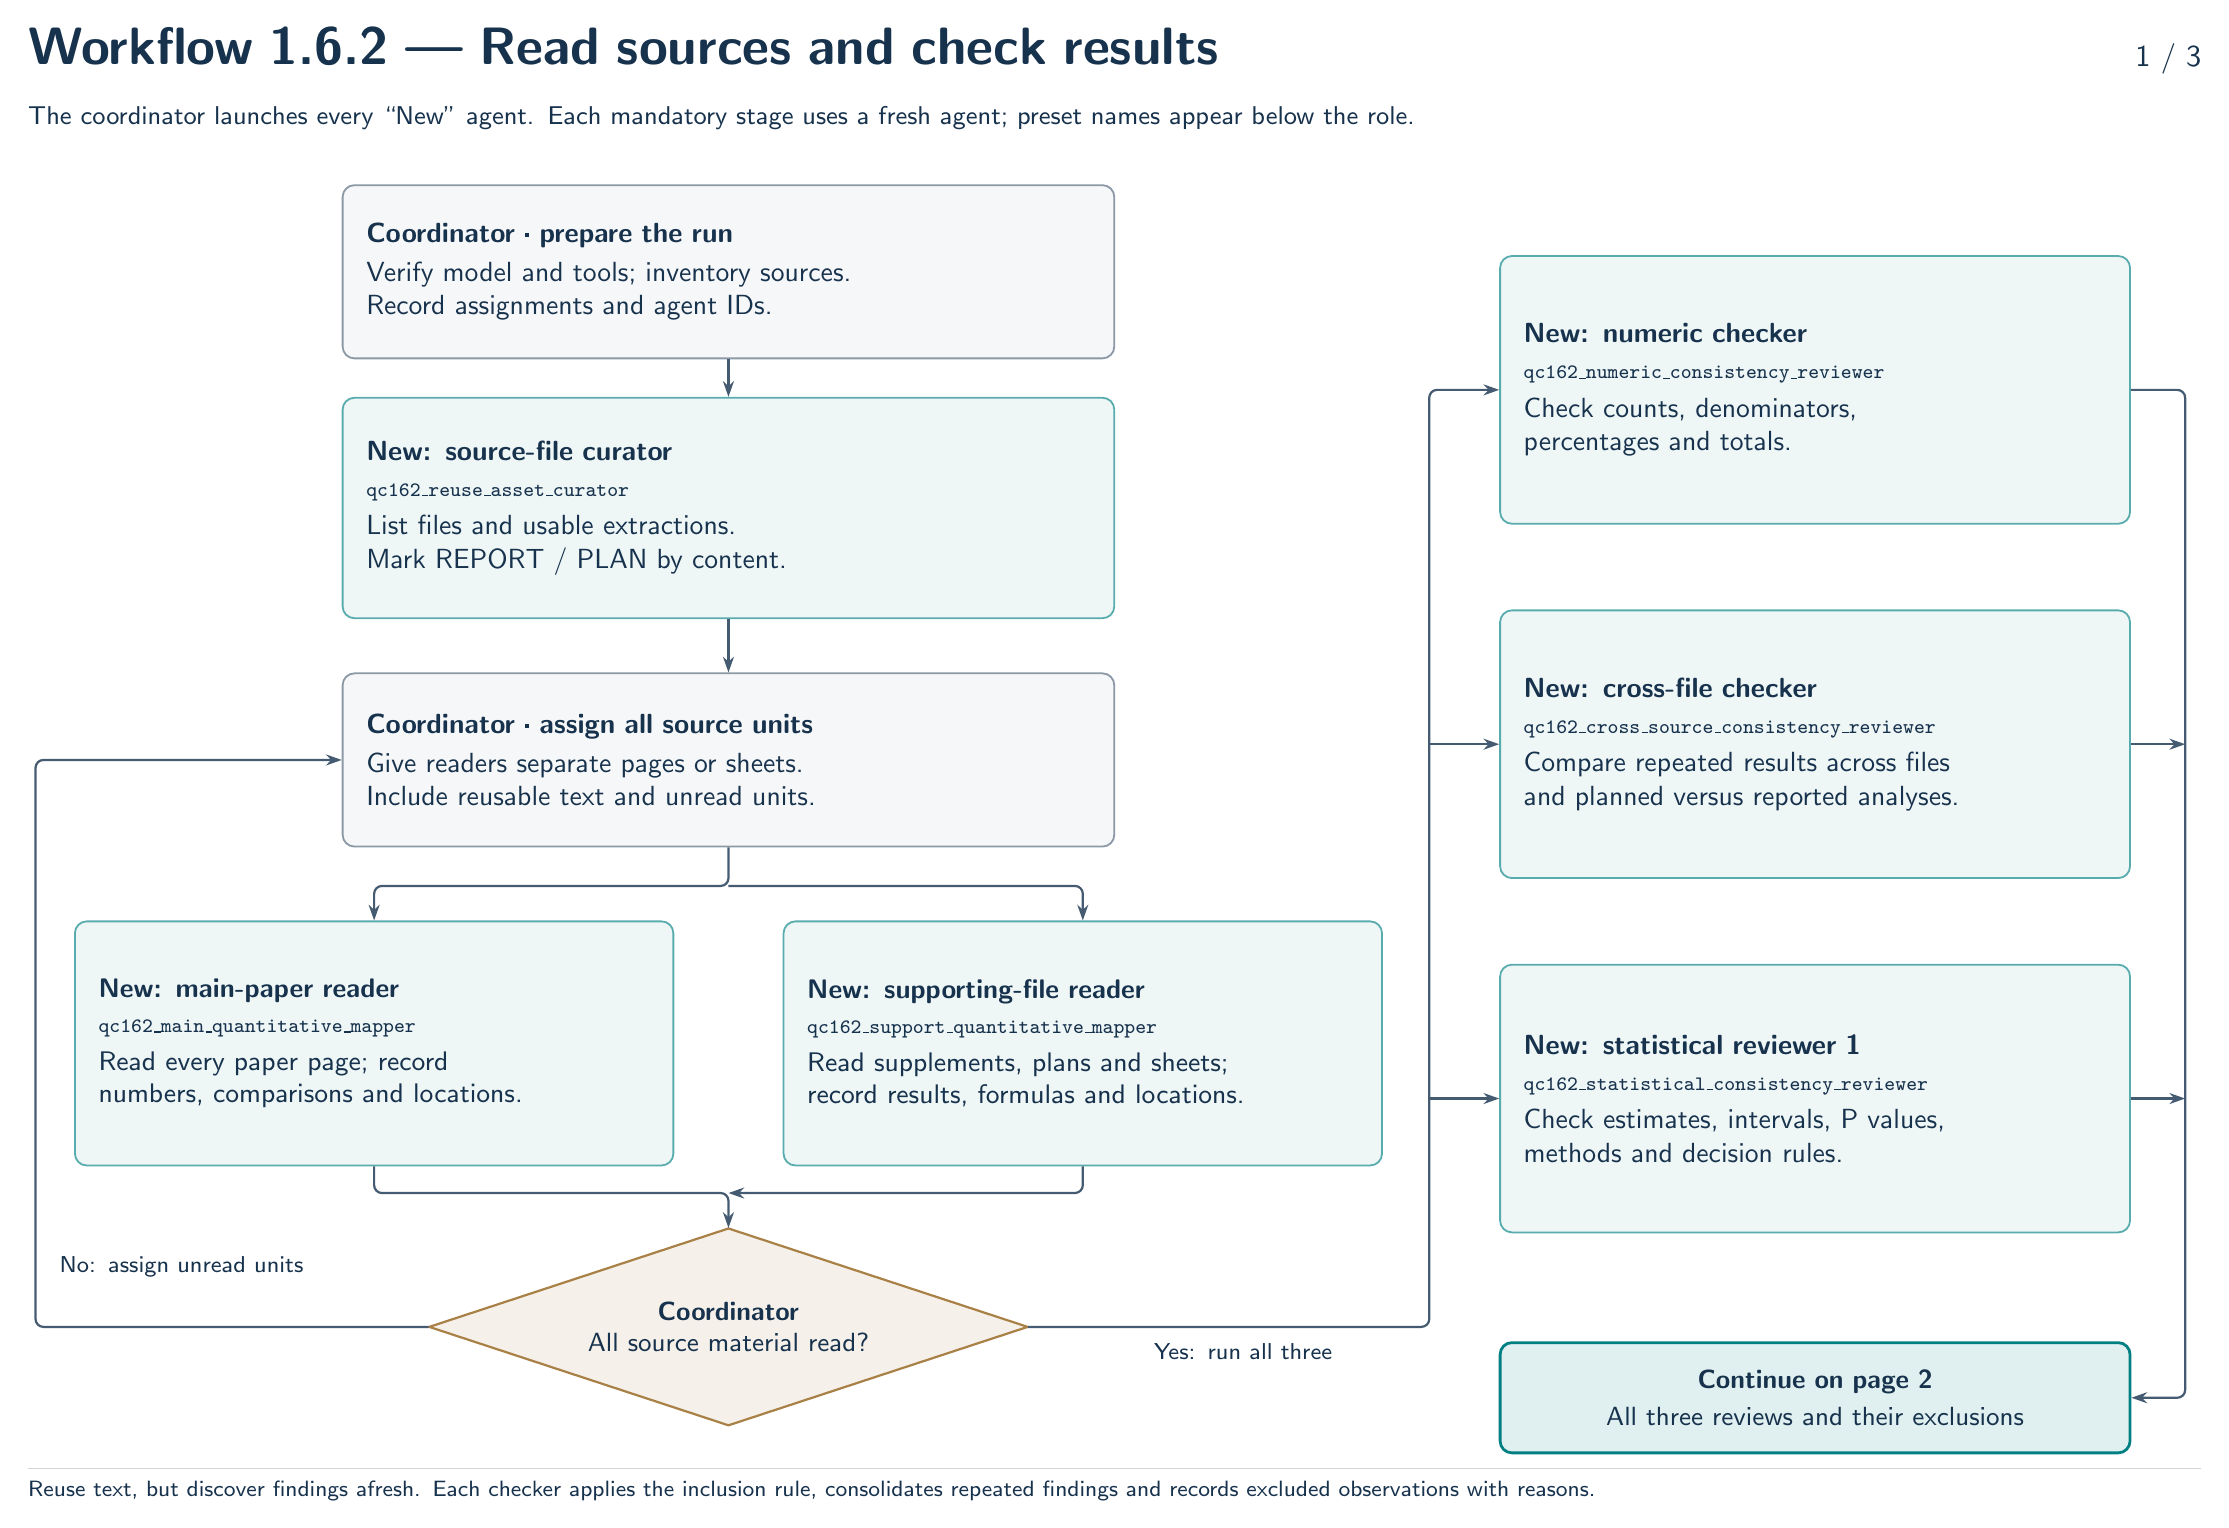
\begin{tikzpicture}[x=1mm,y=-1mm]
\path[use as bounding box] (0,0) rectangle (276,187);
\node[anchor=north west,align=left,text=Navy,text width=253mm,font=\fontsize{19}{21}\selectfont,inner sep=0] at (0,0) {{\fontsize{19}{22}\selectfont\bfseries Workflow 1.6.2 | Read sources and check results}};
\node[anchor=north west,align=left,text=Navy,text width=17mm,font=\fontsize{11}{13}\selectfont,inner sep=0] at (259,2) {\hfill 1 / 3};
\node[anchor=north west,align=left,text=Navy,text width=274mm,font=\fontsize{9.3}{11.3}\selectfont,inner sep=0] at (0,10) {The coordinator launches every “New” agent. Each mandatory stage uses a fresh agent; preset names appear below the role.};
\begin{scope}[shift={(0,20)}]
\node[coord,text width=92mm,minimum width=98mm,minimum height=22mm,font=\fontsize{10}{12}\selectfont] (setup) at (89,11) {\textbf{Coordinator · prepare the run}\\[2pt]Verify model and tools; inventory sources.\\Record assignments and agent IDs.};
\node[box,text width=92mm,minimum width=98mm,minimum height=28mm,font=\fontsize{10}{12}\selectfont] (curator) at (89,41) {\textbf{New: source-file curator}\\[1pt]{\normalfont\ttfamily\fontsize{7.4}{8.8}\selectfont qc162\_reuse\_asset\_curator}\\[2pt]List files and usable extractions.\\Mark REPORT / PLAN by content.};
\node[coord,text width=92mm,minimum width=98mm,minimum height=22mm,font=\fontsize{10}{12}\selectfont] (assign) at (89,73) {\textbf{Coordinator · assign all source units}\\[2pt]Give readers separate pages or sheets.\\Include reusable text and unread units.};
\node[box,text width=70mm,minimum width=76mm,minimum height=31mm,font=\fontsize{9.7}{11.7}\selectfont] (main) at (44,109) {\textbf{New: main-paper reader}\\[1pt]{\normalfont\ttfamily\fontsize{7.4}{8.8}\selectfont qc162\_main\_quantitative\_mapper}\\[2pt]Read every paper page; record\\numbers, comparisons and locations.};
\node[box,text width=70mm,minimum width=76mm,minimum height=31mm,font=\fontsize{9.7}{11.7}\selectfont] (support) at (134,109) {\textbf{New: supporting-file reader}\\[1pt]{\normalfont\ttfamily\fontsize{7.4}{8.8}\selectfont qc162\_support\_quantitative\_mapper}\\[2pt]Read supplements, plans and sheets;\\record results, formulas and locations.};
\draw[gate] (51.0,145) -- (89,132.5) -- (127.0,145) -- (89,157.5) -- cycle;
\node[align=center,text=Navy,text width=61mm,minimum width=76mm,minimum height=25mm,inner sep=0,font=\fontsize{9.5}{11}\selectfont] (coverage) at (89,145) {\textbf{Coordinator}\\All source material read?};
\node[box,text width=74mm,minimum width=80mm,minimum height=34mm,font=\fontsize{10}{12}\selectfont] (num) at (227,26) {\textbf{New: numeric checker}\\[1pt]{\normalfont\ttfamily\fontsize{7.4}{8.8}\selectfont qc162\_numeric\_consistency\_reviewer}\\[2pt]Check counts, denominators,\\percentages and totals.};
\node[box,text width=74mm,minimum width=80mm,minimum height=34mm,font=\fontsize{10}{12}\selectfont] (cross) at (227,71) {\textbf{New: cross-file checker}\\[1pt]{\normalfont\ttfamily\fontsize{7.4}{8.8}\selectfont qc162\_cross\_source\_consistency\_reviewer}\\[2pt]Compare repeated results across files\\and planned versus reported analyses.};
\node[box,text width=74mm,minimum width=80mm,minimum height=34mm,font=\fontsize{10}{12}\selectfont] (statsone) at (227,116) {\textbf{New: statistical reviewer 1}\\[1pt]{\normalfont\ttfamily\fontsize{7.4}{8.8}\selectfont qc162\_statistical\_consistency\_reviewer}\\[2pt]Check estimates, intervals, P values,\\methods and decision rules.};
\node[end,text width=74mm,minimum width=80mm,minimum height=14mm,font=\fontsize{9.5}{11.5}\selectfont] (p2) at (227,154) {\textbf{Continue on page 2}\\[2pt]All three reviews and their exclusions};
\draw[flow] (setup.south) -- (curator.north);
\draw[flow] (curator.south) -- (assign.north);
\draw[flow] (assign.south) -- (89,89) -- (44,89) -- (main.north);
\draw[flow] (89,89) -- (134,89) -- (support.north);
\draw[flow] (main.south) -- (44,128) -- (89,128) -- (coverage.north);
\draw[flow] (support.south) -- (134,128) -- (89,128);
\draw[flow] (coverage.west) -- (1,145) -- (1,73) -- (assign.west);
\node[anchor=north west,align=left,text=Navy,text width=44mm,font=\fontsize{8.3}{10.3}\selectfont,inner sep=0] at (4,136) {No: assign unread units};
\draw[flow] (coverage.east) -- (178,145) -- (178,26) -- (num.west);
\node[anchor=north west,align=left,text=Navy,text width=31mm,font=\fontsize{8.3}{10.3}\selectfont,inner sep=0] at (143,147) {Yes: run all three};
\draw[flow] (178,71) -- (cross.west);
\draw[flow] (178,116) -- (statsone.west);
\draw[flow] (num.east) -- (274,26) -- (274,154) -- (p2.east);
\draw[flow] (cross.east) -- (274,71);
\draw[flow] (statsone.east) -- (274,116);
\end{scope}
\draw[draw=Navy!20] (0,183) -- (276,183);
\node[anchor=north west,align=left,text=Navy,text width=276mm,font=\fontsize{8}{10}\selectfont,inner sep=0] at (0,184.5) {Reuse text, but discover findings afresh. Each checker applies the inclusion rule, consolidates repeated findings and records excluded observations with reasons.};
\end{tikzpicture}
\newpage
\noindent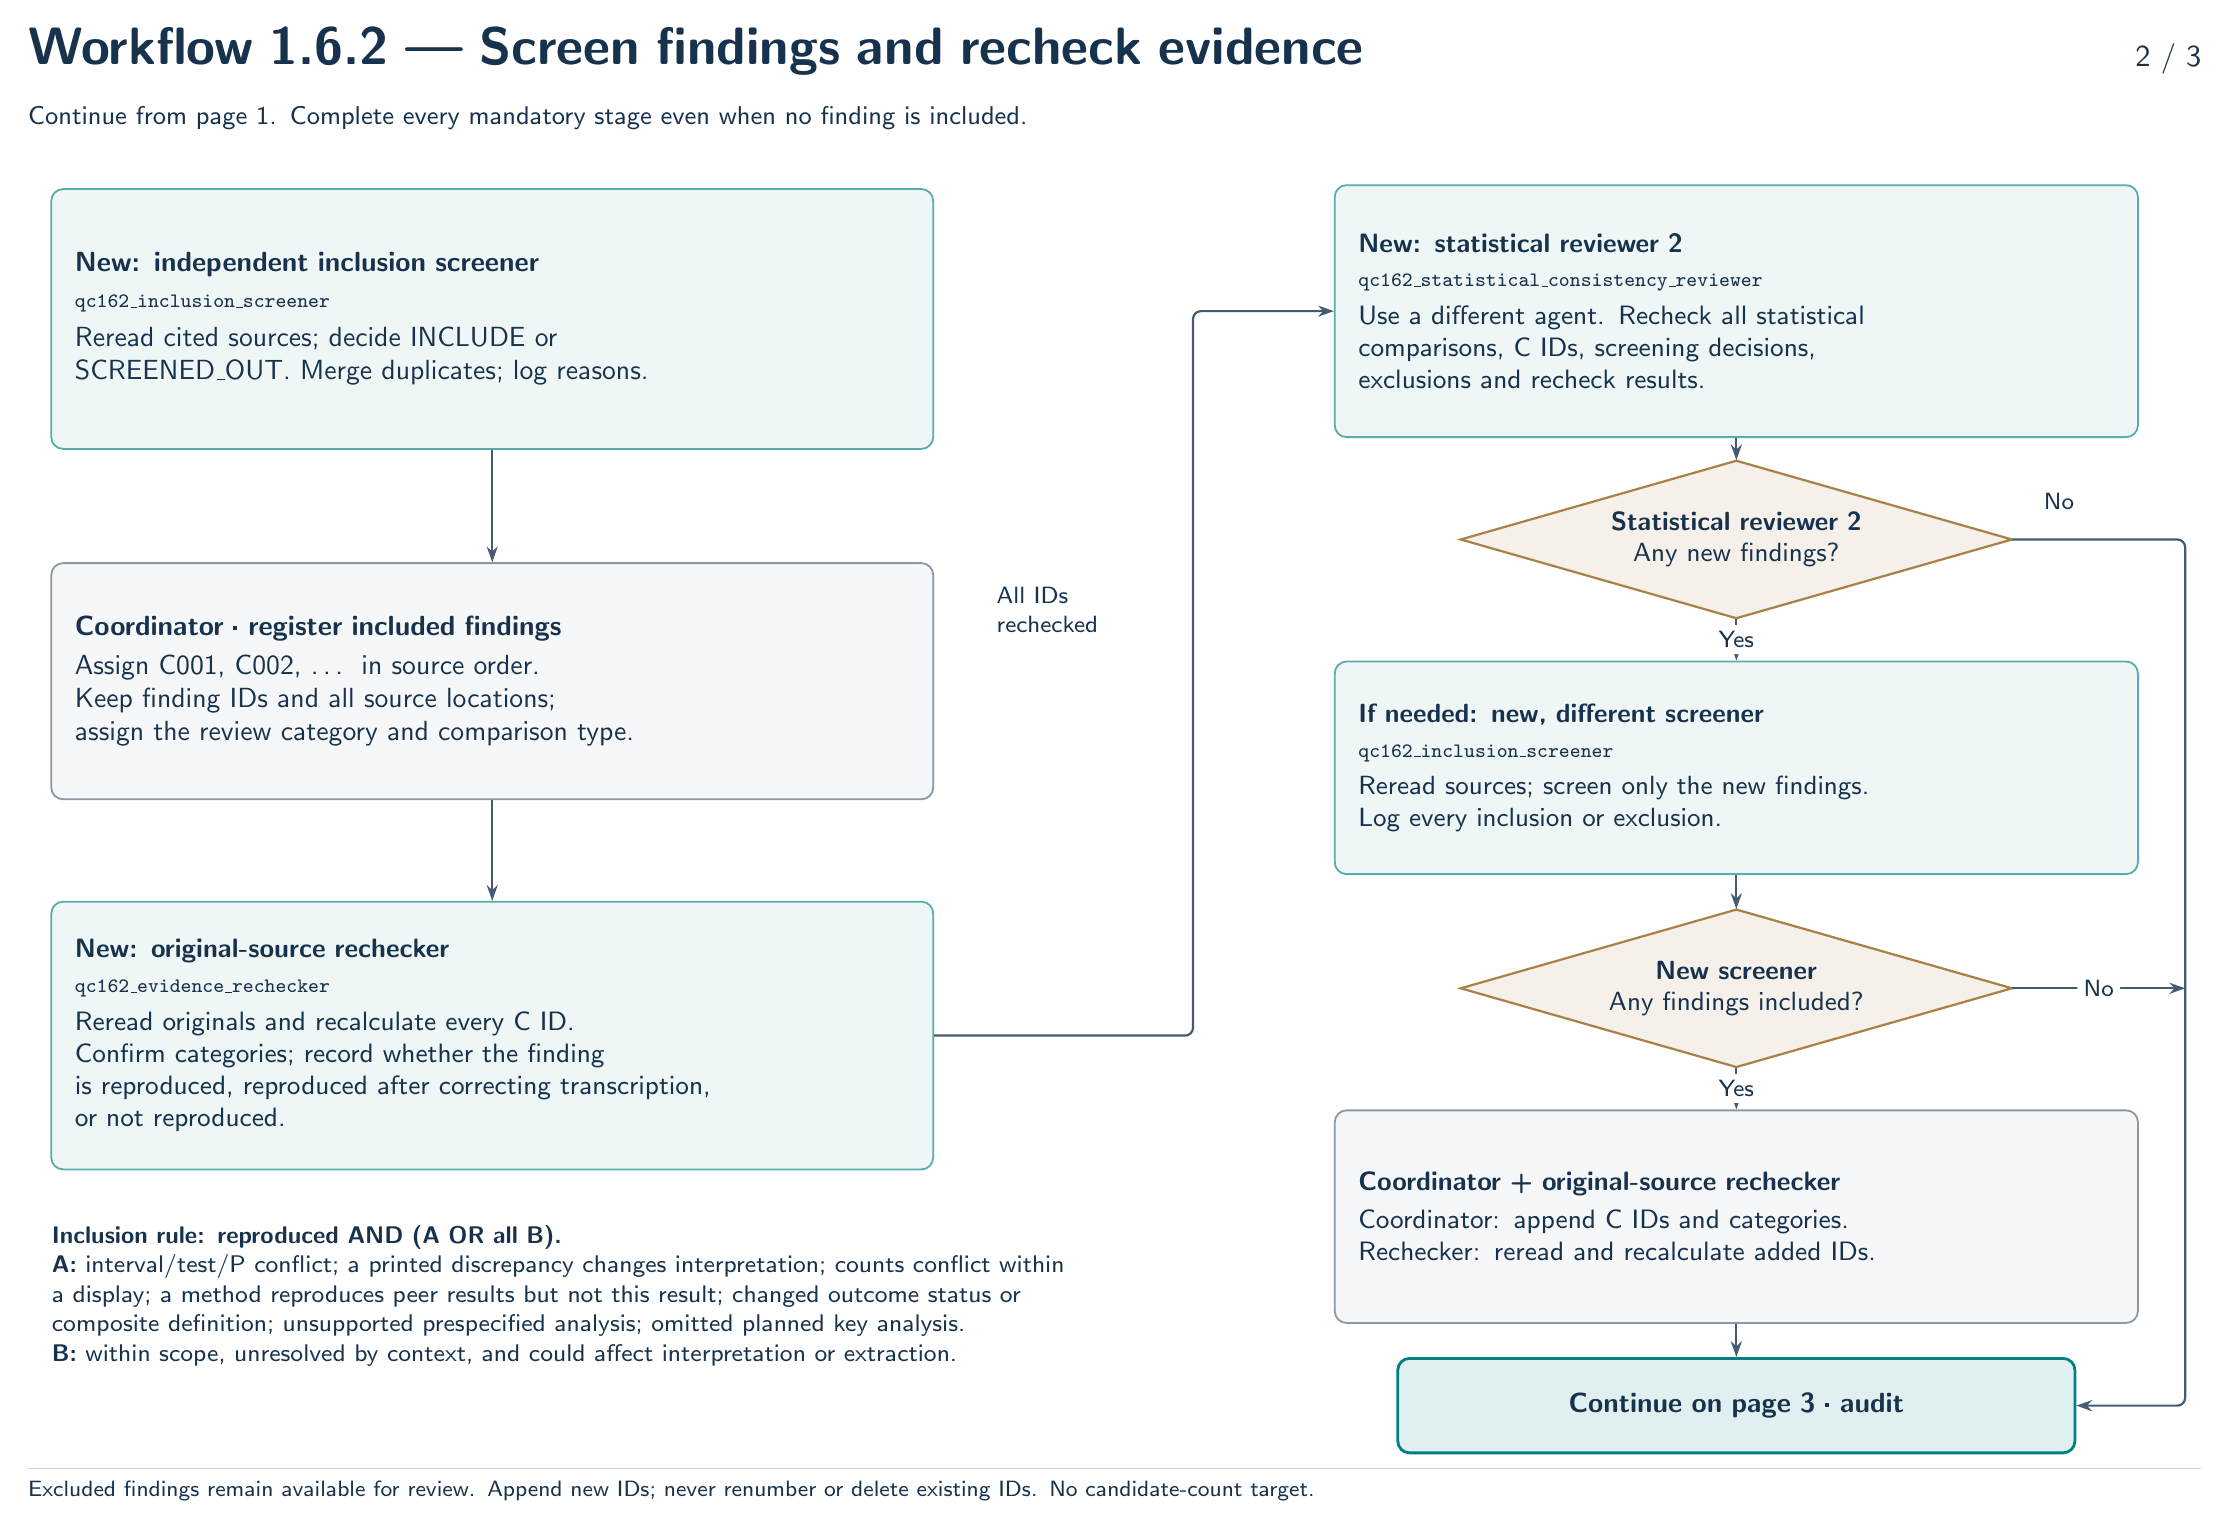
\begin{tikzpicture}[x=1mm,y=-1mm]
\path[use as bounding box] (0,0) rectangle (276,187);
\node[anchor=north west,align=left,text=Navy,text width=253mm,font=\fontsize{19}{21}\selectfont,inner sep=0] at (0,0) {{\fontsize{19}{22}\selectfont\bfseries Workflow 1.6.2 | Screen findings and recheck evidence}};
\node[anchor=north west,align=left,text=Navy,text width=17mm,font=\fontsize{11}{13}\selectfont,inner sep=0] at (259,2) {\hfill 2 / 3};
\node[anchor=north west,align=left,text=Navy,text width=274mm,font=\fontsize{9.3}{11.3}\selectfont,inner sep=0] at (0,10) {Continue from page 1. Complete every mandatory stage even when no finding is included.};
\begin{scope}[shift={(0,20)}]
\node[box,text width=106mm,minimum width=112mm,minimum height=33mm,font=\fontsize{10}{12}\selectfont] (screen) at (59,17) {\textbf{New: independent inclusion screener}\\[1pt]{\normalfont\ttfamily\fontsize{7.4}{8.8}\selectfont qc162\_inclusion\_screener}\\[2pt]Reread cited sources; decide INCLUDE or\\SCREENED\_OUT. Merge duplicates; log reasons.};
\node[coord,text width=106mm,minimum width=112mm,minimum height=30mm,font=\fontsize{10}{12}\selectfont] (register) at (59,63) {\textbf{Coordinator · register included findings}\\[2pt]Assign C001, C002, … in source order.\\Keep finding IDs and all source locations;\\assign the review category and comparison type.};
\node[box,text width=106mm,minimum width=112mm,minimum height=34mm,font=\fontsize{9.6}{11.6}\selectfont] (recheck) at (59,108) {\textbf{New: original-source rechecker}\\[1pt]{\normalfont\ttfamily\fontsize{7.4}{8.8}\selectfont qc162\_evidence\_rechecker}\\[2pt]Reread originals and recalculate every C ID.\\Confirm categories; record whether the finding\\is reproduced, reproduced after correcting transcription,\\or not reproduced.};
\node[box,text width=96mm,minimum width=102mm,minimum height=32mm,font=\fontsize{9.6}{11.6}\selectfont] (statstwo) at (217,16) {\textbf{New: statistical reviewer 2}\\[1pt]{\normalfont\ttfamily\fontsize{7.4}{8.8}\selectfont qc162\_statistical\_consistency\_reviewer}\\[2pt]Use a different agent. Recheck all statistical\\comparisons, C IDs, screening decisions,\\exclusions and recheck results.};
\draw[gate] (182.0,45) -- (217,35.0) -- (252.0,45) -- (217,55.0) -- cycle;
\node[align=center,text=Navy,text width=55mm,minimum width=70mm,minimum height=20mm,inner sep=0,font=\fontsize{9.5}{11}\selectfont] (newfind) at (217,45) {\textbf{Statistical reviewer 2}\\Any new findings?};
\node[box,text width=96mm,minimum width=102mm,minimum height=27mm,font=\fontsize{9.5}{11.5}\selectfont] (secondscreen) at (217,74) {\textbf{If needed: new, different screener}\\[1pt]{\normalfont\ttfamily\fontsize{7.4}{8.8}\selectfont qc162\_inclusion\_screener}\\[2pt]Reread sources; screen only the new findings.\\Log every inclusion or exclusion.};
\draw[gate] (182.0,102) -- (217,92.0) -- (252.0,102) -- (217,112.0) -- cycle;
\node[align=center,text=Navy,text width=55mm,minimum width=70mm,minimum height=20mm,inner sep=0,font=\fontsize{9.5}{11}\selectfont] (included) at (217,102) {\textbf{New screener}\\Any findings included?};
\node[coord,text width=96mm,minimum width=102mm,minimum height=27mm,font=\fontsize{9.6}{11.6}\selectfont] (append) at (217,131) {\textbf{Coordinator + original-source rechecker}\\[2pt]Coordinator: append C IDs and categories.\\Rechecker: reread and recalculate added IDs.};
\node[end,text width=80mm,minimum width=86mm,minimum height=12mm,font=\fontsize{10}{12}\selectfont] (p3) at (217,155) {\textbf{Continue on page 3 · audit}};
\draw[flow] (screen.south) -- (register.north);
\draw[flow] (register.south) -- (recheck.north);
\draw[flow] (recheck.east) -- (148,108) -- (148,16) -- (statstwo.west);
\node[anchor=north west,align=left,text=Navy,text width=20mm,font=\fontsize{8.5}{10.5}\selectfont,inner sep=0] at (123,51) {All IDs\\rechecked};
\draw[flow] (statstwo.south) -- (newfind.north);
\draw[flow] (newfind.south) -- (secondscreen.north) node[tag,midway] {Yes};
\draw[flow] (secondscreen.south) -- (included.north);
\draw[flow] (included.south) -- (append.north) node[tag,midway] {Yes};
\draw[flow] (append.south) -- (p3.north);
\draw[flow] (newfind.east) -- (274,45) -- (274,155) -- (p3.east);
\node[anchor=north west,align=left,text=Navy,text width=16mm,font=\fontsize{8.5}{10.5}\selectfont,inner sep=0] at (256,39) {No};
\draw[flow] (included.east) -- (274,102) node[tag,midway] {No};
\node[anchor=north west,align=left,text=Navy,text width=130mm,font=\fontsize{8.7}{10.7}\selectfont,inner sep=0] at (3,132) {\textbf{Inclusion rule: reproduced AND (A OR all B).}\\\textbf{A:} interval/test/P conflict; a printed discrepancy changes interpretation; counts conflict within a display; a method reproduces peer results but not this result; changed outcome status or composite definition; unsupported prespecified analysis; omitted planned key analysis.\\\textbf{B:} within scope, unresolved by context, and could affect interpretation or extraction.};
\end{scope}
\draw[draw=Navy!20] (0,183) -- (276,183);
\node[anchor=north west,align=left,text=Navy,text width=276mm,font=\fontsize{8}{10}\selectfont,inner sep=0] at (0,184.5) {Excluded findings remain available for review. Append new IDs; never renumber or delete existing IDs. No candidate-count target.};
\end{tikzpicture}
\newpage
\noindent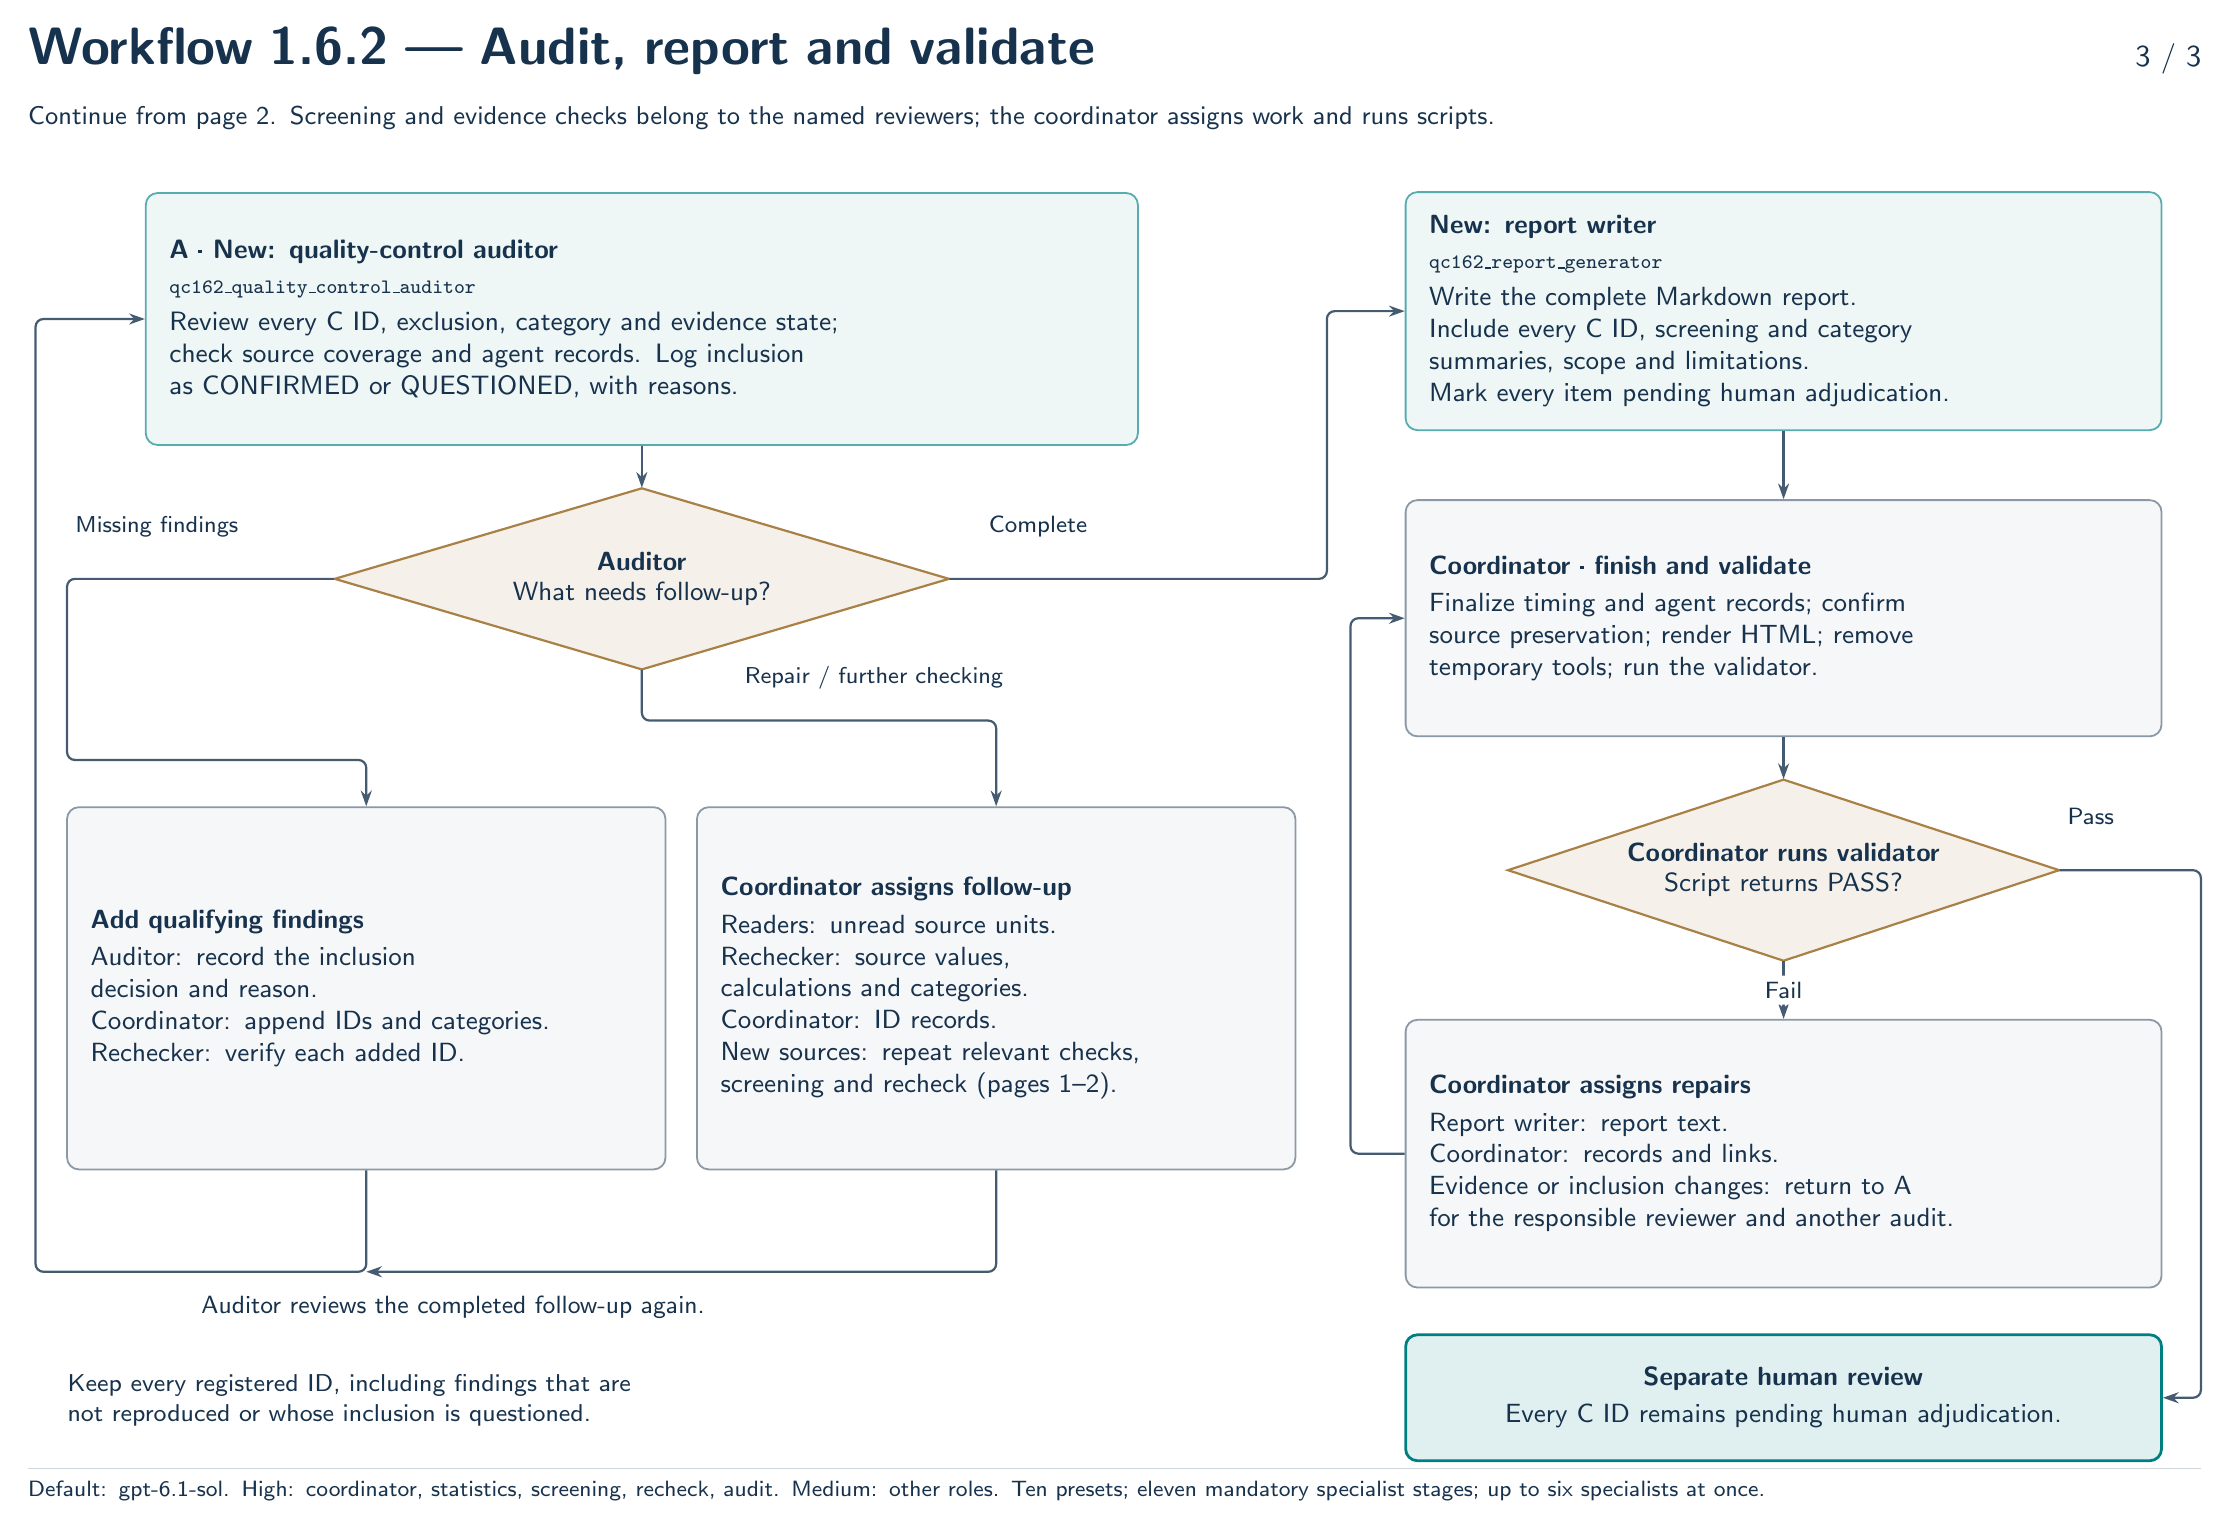
\begin{tikzpicture}[x=1mm,y=-1mm]
\path[use as bounding box] (0,0) rectangle (276,187);
\node[anchor=north west,align=left,text=Navy,text width=253mm,font=\fontsize{19}{21}\selectfont,inner sep=0] at (0,0) {{\fontsize{19}{22}\selectfont\bfseries Workflow 1.6.2 | Audit, report and validate}};
\node[anchor=north west,align=left,text=Navy,text width=17mm,font=\fontsize{11}{13}\selectfont,inner sep=0] at (259,2) {\hfill 3 / 3};
\node[anchor=north west,align=left,text=Navy,text width=274mm,font=\fontsize{9.3}{11.3}\selectfont,inner sep=0] at (0,10) {Continue from page 2. Screening and evidence checks belong to the named reviewers; the coordinator assigns work and runs scripts.};
\begin{scope}[shift={(0,20)}]
\node[box,text width=120mm,minimum width=126mm,minimum height=32mm,font=\fontsize{9.6}{11.6}\selectfont] (audit) at (78,17) {\textbf{A · New: quality-control auditor}\\[1pt]{\normalfont\ttfamily\fontsize{7.4}{8.8}\selectfont qc162\_quality\_control\_auditor}\\[2pt]Review every C ID, exclusion, category and evidence state;\\check source coverage and agent records. Log inclusion\\as CONFIRMED or QUESTIONED, with reasons.};
\draw[gate] (39.0,50) -- (78,38.5) -- (117.0,50) -- (78,61.5) -- cycle;
\node[align=center,text=Navy,text width=63mm,minimum width=78mm,minimum height=23mm,inner sep=0,font=\fontsize{9.5}{11}\selectfont] (auditdecision) at (78,50) {\textbf{Auditor}\\What needs follow-up?};
\node[coord,text width=70mm,minimum width=76mm,minimum height=46mm,font=\fontsize{9.5}{11.5}\selectfont] (rescue) at (43,102) {\textbf{Add qualifying findings}\\[2pt]Auditor: record the inclusion\\decision and reason.\\Coordinator: append IDs and categories.\\Rechecker: verify each added ID.};
\node[coord,text width=70mm,minimum width=76mm,minimum height=46mm,font=\fontsize{9.5}{11.5}\selectfont] (auditfix) at (123,102) {\textbf{Coordinator assigns follow-up}\\[2pt]Readers: unread source units.\\Rechecker: source values,\\calculations and categories.\\Coordinator: ID records.\\New sources: repeat relevant checks,\\screening and recheck (pages 1–2).};
\node[box,text width=90mm,minimum width=96mm,minimum height=30mm,font=\fontsize{9.5}{11.5}\selectfont] (report) at (223,16) {\textbf{New: report writer}\\[1pt]{\normalfont\ttfamily\fontsize{7.4}{8.8}\selectfont qc162\_report\_generator}\\[2pt]Write the complete Markdown report.\\Include every C ID, screening and category\\summaries, scope and limitations.\\Mark every item pending human adjudication.};
\node[coord,text width=90mm,minimum width=96mm,minimum height=30mm,font=\fontsize{9.5}{11.5}\selectfont] (render) at (223,55) {\textbf{Coordinator · finish and validate}\\[2pt]Finalize timing and agent records; confirm\\source preservation; render HTML; remove\\temporary tools; run the validator.};
\draw[gate] (188.0,87) -- (223,75.5) -- (258.0,87) -- (223,98.5) -- cycle;
\node[align=center,text=Navy,text width=55mm,minimum width=70mm,minimum height=23mm,inner sep=0,font=\fontsize{9.5}{11}\selectfont] (pass) at (223,87) {\textbf{Coordinator runs validator}\\Script returns PASS?};
\node[coord,text width=90mm,minimum width=96mm,minimum height=34mm,font=\fontsize{9.5}{11.5}\selectfont] (filefix) at (223,123) {\textbf{Coordinator assigns repairs}\\[2pt]Report writer: report text.\\Coordinator: records and links.\\Evidence or inclusion changes: return to A\\for the responsible reviewer and another audit.};
\node[end,text width=90mm,minimum width=96mm,minimum height=16mm,font=\fontsize{9.5}{11.5}\selectfont] (human) at (223,154) {\textbf{Separate human review}\\[2pt]Every C ID remains pending human adjudication.};
\draw[flow] (audit.south) -- (auditdecision.north);
\draw[flow] (auditdecision.west) -- (5,50) -- (5,73) -- (43,73) -- (rescue.north);
\node[anchor=north west,align=left,text=Navy,text width=32mm,font=\fontsize{8.3}{10.3}\selectfont,inner sep=0] at (6,42) {Missing findings};
\draw[flow] (auditdecision.south) -- (78,68) -- (123,68) -- (auditfix.north);
\node[anchor=north west,align=left,text=Navy,text width=63mm,font=\fontsize{8.3}{10.3}\selectfont,inner sep=0] at (91,61) {Repair / further checking};
\draw[flow] (rescue.south) -- (43,138) -- (1,138) -- (1,17) -- (audit.west);
\draw[flow] (auditfix.south) -- (123,138) -- (43,138);
\node[anchor=north west,align=left,text=Navy,text width=133mm,font=\fontsize{9}{11}\selectfont,inner sep=0] at (22,141) {Auditor reviews the completed follow-up again.};
\node[anchor=north west,align=left,text=Navy,text width=151mm,font=\fontsize{8.8}{10.8}\selectfont,inner sep=0] at (5,151) {Keep every registered ID, including findings that are\\not reproduced or whose inclusion is questioned.};
\draw[flow] (auditdecision.east) -- (165,50) -- (165,16) -- (report.west);
\node[anchor=north west,align=left,text=Navy,text width=40mm,font=\fontsize{8.5}{10.5}\selectfont,inner sep=0] at (122,42) {Complete};
\draw[flow] (report.south) -- (render.north);
\draw[flow] (render.south) -- (pass.north);
\draw[flow] (pass.south) -- (filefix.north) node[tag,midway] {Fail};
\draw[flow] (filefix.west) -- (168,123) -- (168,55) -- (render.west);
\draw[flow] (pass.east) -- (276,87) -- (276,154) -- (human.east);
\node[anchor=north west,align=left,text=Navy,text width=16mm,font=\fontsize{8.5}{10.5}\selectfont,inner sep=0] at (259,79) {Pass};
\end{scope}
\draw[draw=Navy!20] (0,183) -- (276,183);
\node[anchor=north west,align=left,text=Navy,text width=276mm,font=\fontsize{8}{10}\selectfont,inner sep=0] at (0,184.5) {Default: gpt-6.1-sol. High: coordinator, statistics, screening, recheck, audit. Medium: other roles. Ten presets; eleven mandatory specialist stages; up to six specialists at once.};
\end{tikzpicture}
\end{document}
